\documentclass[conference]{IEEEtran}
\IEEEoverridecommandlockouts
% The preceding line is only needed to identify funding in the first footnote. If that is unneeded, please comment it out.
\usepackage{cite}
\usepackage{amsmath,amssymb,amsfonts}
\usepackage{algorithmic}
\usepackage{graphicx}
\usepackage{textcomp}
\usepackage{xcolor}
\usepackage{hyperref}
\def\BibTeX{{\rm B\kern-.05em{\sc i\kern-.025em b}\kern-.08em
    T\kern-.1667em\lower.7ex\hbox{E}\kern-.125emX}}
%\usepackage{biblatex}
    
%encoding
%--------------------------------------
\usepackage[T1]{fontenc}
\usepackage[utf8]{inputenc}
%--------------------------------------

%Portuguese-specific commands
%--------------------------------------
\usepackage[portuguese]{babel}
%--------------------------------------

%Hyphenation rules
%--------------------------------------
\usepackage{hyphenat}
\hyphenation{mate-mática recu-perar}
%--------------------------------------  
    
\begin{document}

\title{COVID-19 na População Mundial\\
}

\author{\IEEEauthorblockN{Bruno Carvalho}
\IEEEauthorblockA{\textit{Departamento de Engenharia Informática} \\
\textit{Instituto Superior de Engenharia do Porto}\\
Porto, Portugal \\
1200145@isep.ipp.pt}
\and
\IEEEauthorblockN{Sofia Canelas}
\IEEEauthorblockA{\textit{Departamento de Engenharia Informática} \\
\textit{Instituto Superior de Engenharia do Porto}\\
Porto, Portugal \\
1200185@isep.ipp.pt}
}

\maketitle

\begin{abstract}
Através de dados retirados de uma base de dados internacional, pretende-se analisar o impacto da pandemia na população mundial seguindo processos de análise exploratória de dados, análise inferencial e análise de correlação e regressão.
\end{abstract}

\begin{IEEEkeywords}
análise, dados, estatística, COVID-19, pandemia, exploração, inferência, correlação, regressão
\end{IEEEkeywords}

\section{Introdução} 
No âmbito da pandemia atual, foram extraídos da base de dados internacional Our World in Data \cite{database}, dinamizada pela Johns Hopkins University (JHU), dados reais incidentes em casos confirmados de COVID-19, taxa de transmissibilidade do vírus, mortes, pacientes nos cuidados intensivos, testagem, vacinação e dados acerca da população. Estes dados são referentes ao período entre 01 de janeiro de 2020 a 27 de fevereiro de 2021.

Pretende-se analisar o impacto da pandemia na população mundial, com o objetivo de compreender a expansão e tratamento do vírus em diferentes partes do mundo. Irá destacar-se a análise do número de mortes ocorridas, o número total de infetados, a taxa de transmissibilidade do vírus, entre outros fatores exploratórios. Estes dados serão discutidos através de processos de análise exploratória de dados, análise inferencial e análise de correlação e regressão.


\section{Metodologia de Trabalho}
Tendo por base o ficheiro “owid-covid-data.csv”\cite{dataFile}, foi criado um script em R com quatro diferentes tipos de análise: Análise Exploratória de Dados, Análise Inferencial, Análise de Correlação e Análise de Regressão. Cada uma destas análises possui alíneas independentes que pretendem tratar de dados específicos referentes ao ficheiro de dados. Após a conclusão das diferentes alíneas, foram analisados os dados e tiradas as respetivas conclusões presentes neste artigo nas secções IV, V, VI e VII.

\section{Exploração e Preparação dos Dados}
No início do script em R estão presentes as variáveis globais que permitem facilitar a obtenção de dados necessários às diversas análises realizadas. Estas tiveram como função guardar os nomes, códigos e cores dos continentes e países necessários à exploração de dados pretendida. Para além disso, está também presente a importação de duas bibliotecas: \textit{nortest} \cite{nortest} e \textit{car} \cite{car}, que permitem a realização de diversos testes presentes nas análises efetuadas. 

O script está organizado pelas análises, delimitadas de forma evidente, sendo que cada uma destas contém várias alíneas, listadas alfabeticamente. As letras indicadoras das alíneas são correspondentes às letras que delimitam as respetivas secções de análise neste artigo.  Em cada alínea existe uma secção para a criação de variáveis referentes à própria alínea (ou mais do que uma alínea, caso os dados se repitam), seguidas da seleção dos dados conforme o pretendido, assim como modificações aos mesmos, caso necessário (por exemplo, a remoção de NAs ou organização dos dados). 

Em seguida, é visível o código que permite a realização da respetiva análise, o qual inclui a criação de gráficos ou testes estatísticos. Nos gráficos que possuem diferentes amostras de populações, deu-se uso a paletas de cor \cite{colors}, de modo a facilitar a visualização dos mesmos. Já os testes estatísticos, são visíveis na consola do script e referidos ao longo do artigo.


\section{Análise Exploratória de Dados} %-------------------------------------

Na análise exploratória de dados pretendeu-se analisar diversas características referentes aos continentes e determinados países, como o número de infetados, número de mortes e taxa de transmissibilidade do vírus.

\subsection{Número total de infetados ao longo do período de tempo estabelecido, por continente}

\begin{figure}[htbp]
\centerline{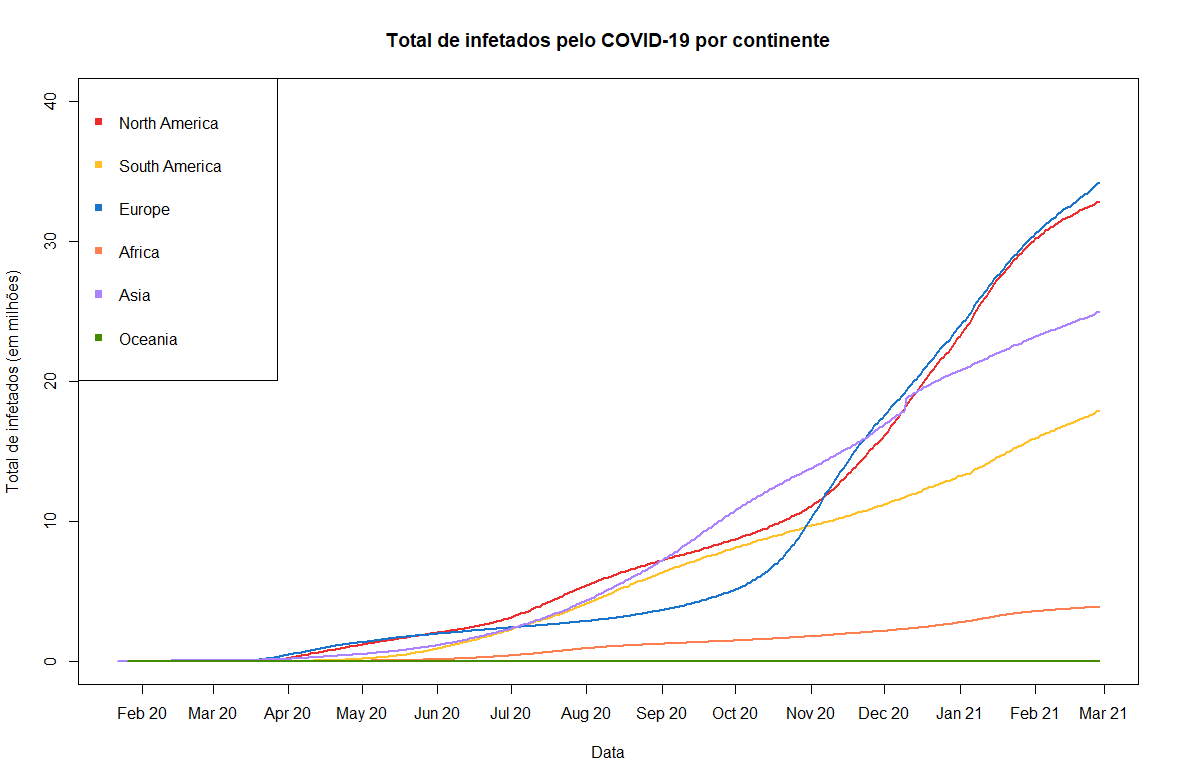
\includegraphics[width=0.95\columnwidth]{images/01.a.png}}
\caption{Gráfico de linhas representativo do total de infetados pelo COVID-19, por continente, ao longo do período de tempo estabelecido}
\label{1a}
\end{figure}

No gráfico de linhas da Fig.\ref{1a} observa-se que a América do Norte e Europa são os continentes que se destacam com os valores mais elevados de infetados, tendo ambos registado uma subida acentuada a partir dos meses de outubro e novembro, onde a Europa registou mais de 34 milhões de infetados. 

Relativamente à Ásia e América do Sul, estes apresentam uma subida regular a partir de maio, sendo que a Ásia se distanciou com mais casos registados desde setembro.

Em contrapartida, África apresenta valores relativamente baixos em relação aos continentes referidos e a Oceânia destaca-se com um número reduzido de casos detetados durante todo o período apresentado no gráfico, com um máximo registado de quase 33.000 casos de infeção por COVID-19.


\subsection{Número total de infetados por milhão de habitantes, ao longo do período de tempo, por continente}

\begin{figure}[htbp]
\centerline{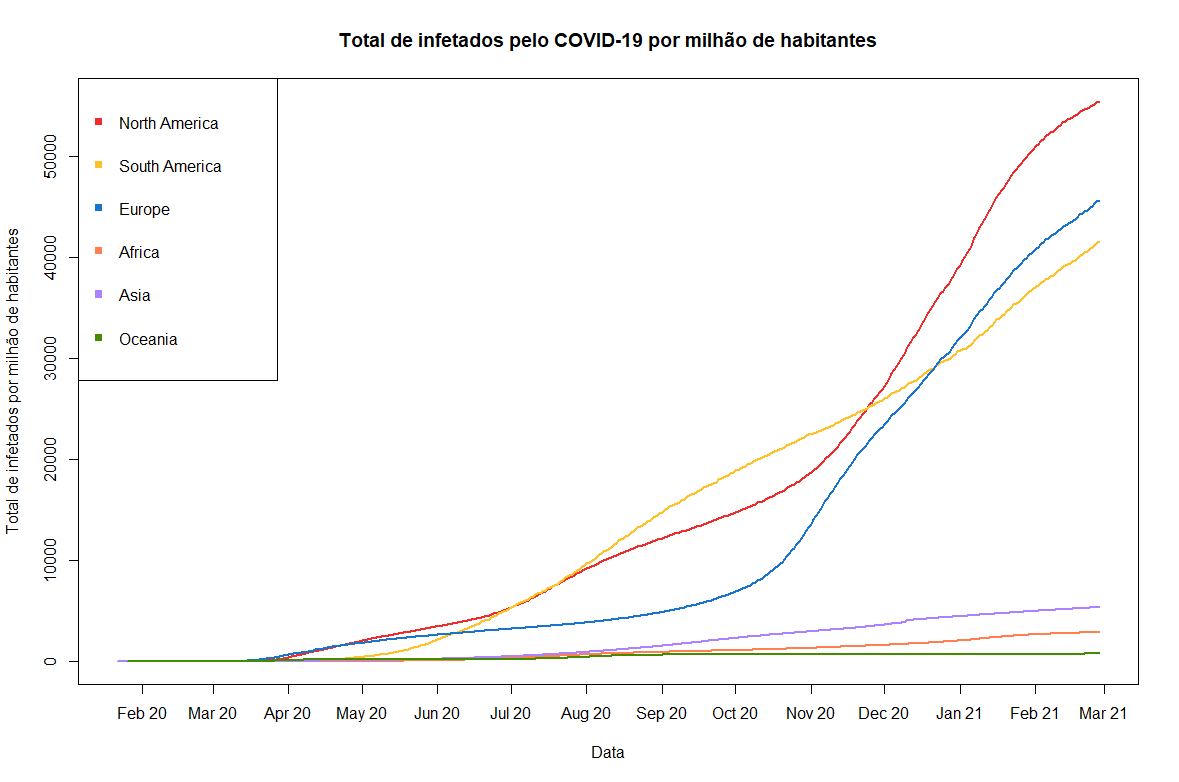
\includegraphics[width=0.95\columnwidth]{images/01.b.png}}
\caption{Gráfico de linhas representativo do total de infetados pelo COVID-19 por milhão de habitantes, por continente, ao longo do período de tempo estabelecido}
\label{1b}
\end{figure}

Neste gráfico de linhas da Fig.\ref{1b} conclui-se que a América do Norte é o continente que possui maior número total de infetados por milhão de habitantes, ultrapassando os 50.000 milhões de habitantes. Por outro lado, a Oceânia é, não só o continente mais estável uma vez que não se verificam oscilações significativas no número de infetados, como também é o que está mais próximo do 0, ou seja, é o continente com menor número de infetados por milhão de habitante.

É de notar que a América e a Europa são os únicos a ultrapassar o valor de 10.000 milhões de habitantes e cujas linhas tendem a subir de forma exponencial, ao contrário dos restantes continentes que se mantêm abaixo desse patamar e cujo crescimento é mais linear.


\subsection{Número de mortos diários, por milhão de habitantes, dos seguintes países: Portugal, Espanha, Itália e Reino Unido}

\begin{figure}[htbp]
\centerline{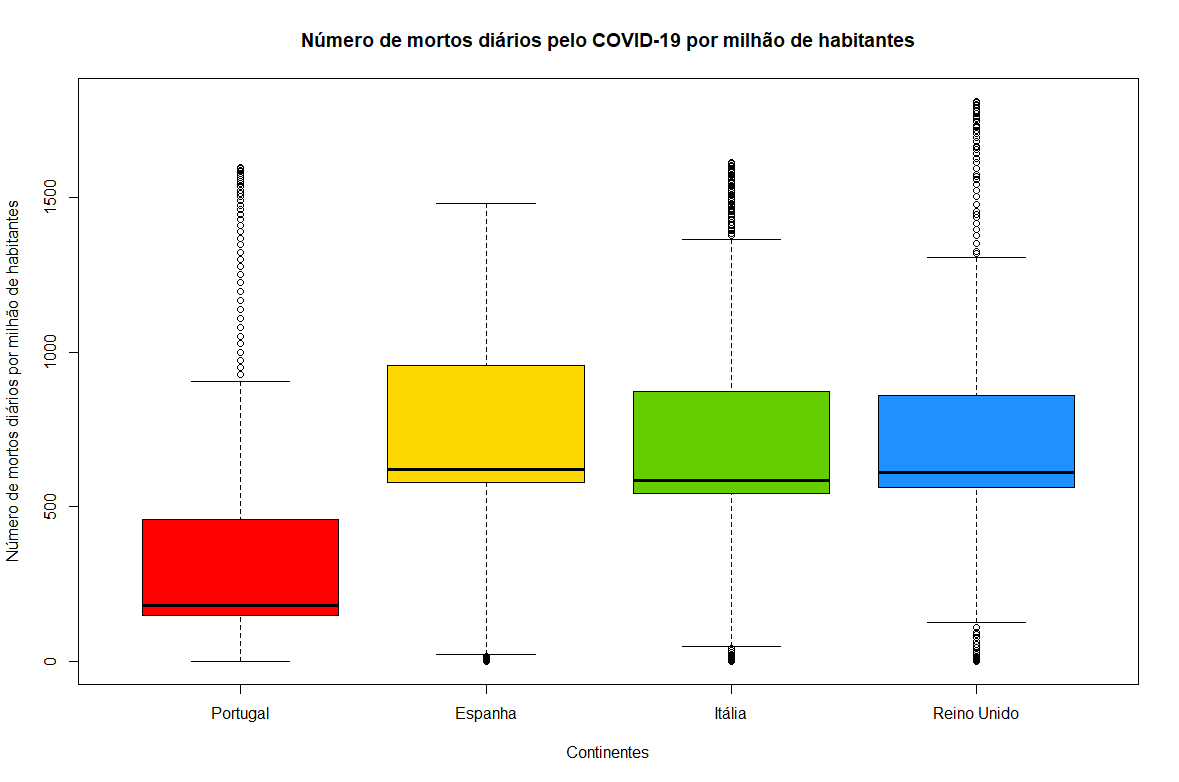
\includegraphics[width=0.95\columnwidth]{images/01.c.png}}
\caption{Diagrama de Caixa representativo do número de mortos diário pelo COVID-19 por milhão de habitantes, em Portugal, Espanha, Itália e Reino Unido}
\label{1c}
\end{figure}

O diagrama de caixa presente na Fig.\ref{1c}, demonstra, no geral, que Portugal, Itália e o Reino Unido têm amplitudes interquartis semelhantes, com Espanha um pouco acima destes três países. Também é possível observar que todos os países presentes nesta análise apresentam uma assimetria negativa, onde a mediana se encontra na parte inferior das caixas.

Espanha é o país com maior número de mortes diárias, por milhão de habitantes, e, também, o que apresenta maior discrepância dos dados, no entanto, sem apresentar \textit{outliers} acima do terceiro quartil, ou seja, não registou nenhum dia com mortes acima da normalidade dos dados.

Em contrapartida, Portugal apresenta números mais reduzidos em relação aos restantes, com a particularidade de ter \textit{outliers} acima do terceiro quartil, o que representa que, em vários dias, Portugal teve um número de mortes diárias significativamente acima da maioria do período temporal dos dados registados.

Em relação a Itália e Inglaterra, estes apresentam dados bastante semelhantes, onde a maior diferença encontra-se no elevado número de outliers acima do terceiro quartil.


\subsection{Número total de mortos, por milhão de habitantes, e o número de testes diários, por milhar de habitantes, dos países: Albânia, Dinamarca, Alemanha e Rússia}

\begin{figure}[htbp]
\centerline{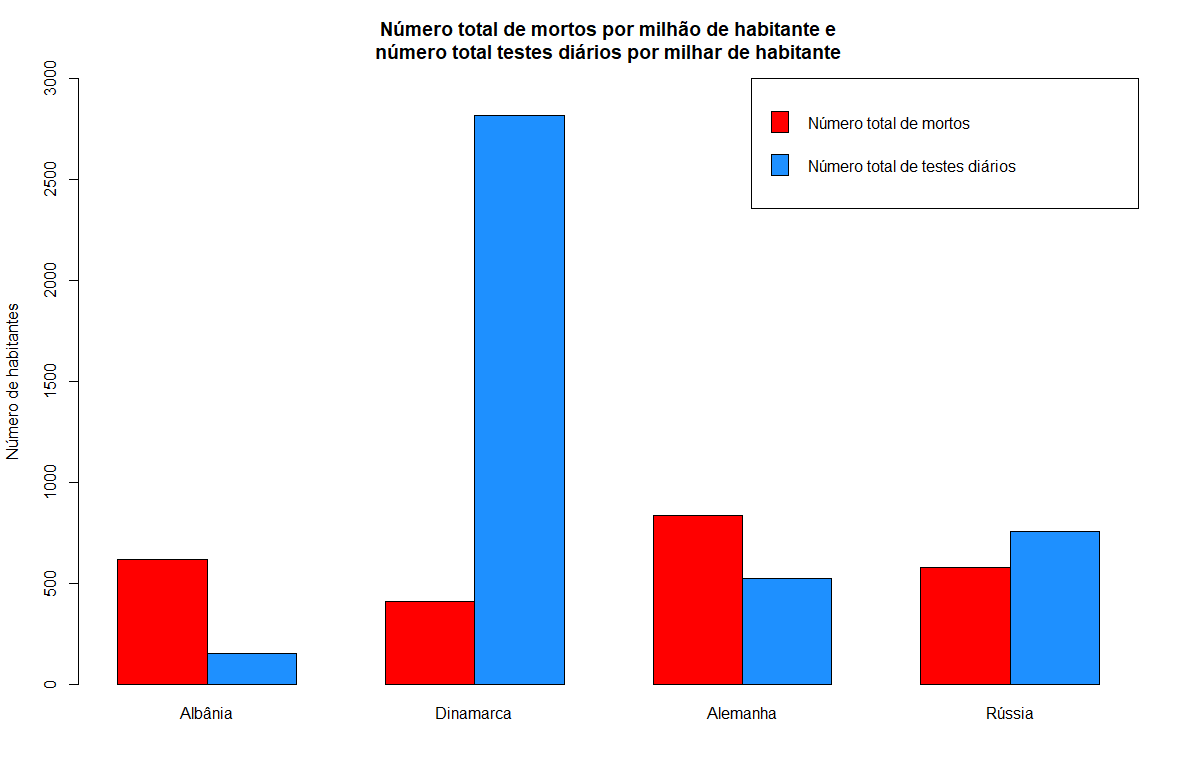
\includegraphics[width=0.95\columnwidth]{images/01.d.png}}
\caption{Gráfico de Barras representativo do número total de mortos pelo COVID-19 por milhão de habitantes, e número de testes diários por milhar de habitantes, na Albânia, Dinamarca, Alemanha e Rússia}
\label{1d}
\end{figure}

Como se observa no gráfico de barras da Fig.\ref{1d}, a Dinamarca destaca-se como o país com maior número total de testes diários em relação aos outros presentes nesta análise, com um máximo superior a 2.800 pessoas testadas por cada milhar de habitante. Contrastando, a Albânia possui o menor número de testes, tendo atingido pouco mais de 150 pessoas testadas, por milhar de habitantes, num único dia. Relativamente à Alemanha e Rússia, estes encontram-se entre os 500 e 1.000 testes diários, nos seus melhores dias de testagem. 

A nível do número total de mortos, a Dinamarca volta a destacar-se como o país com o número mais reduzido, tendo aproximadamente um total de 400 mortos. O número mais notório encontra-se na Alemanha, com um valor acima 800 mortos, o dobro dos registos da Dinamarca. Os valores obtidos da Albânia e Rússia rondam um total de 600 mortos, por milhão de habitantes. 

Assim, percebe-se que a Dinamarca é o país com maior destaque destes quatro, sendo aquele com maior número de testes realizados num dia e menor número total de mortos. Também é possível concluir que a Alemanha e Rússia apresentam valores relativamente próximos nestes dois parâmetros e a Albânia demonstra uma discrepância significativa.


\subsection{País europeu com maior número de infetados, por milhão de habitantes, num único dia}
O Vaticano registou um total de 8.652,658/1.000.000 de habitantes infetados no dia 12 de outubro de 2020, sendo, assim, o país europeu com maior número de infetados, por milhão de habitante, num único dia. 

\subsection{Dia e país onde se registou a maior taxa de transmissibilidade do vírus}
A Coreia do Sul registou, no dia 22 de fevereiro de 2020, a maior taxa de transmissibilidade do vírus, sendo esse valor de 6,72. 

\subsection{Número de mortos diários por milhão de habitantes, em cada continente}

\begin{figure}[htbp]
\centerline{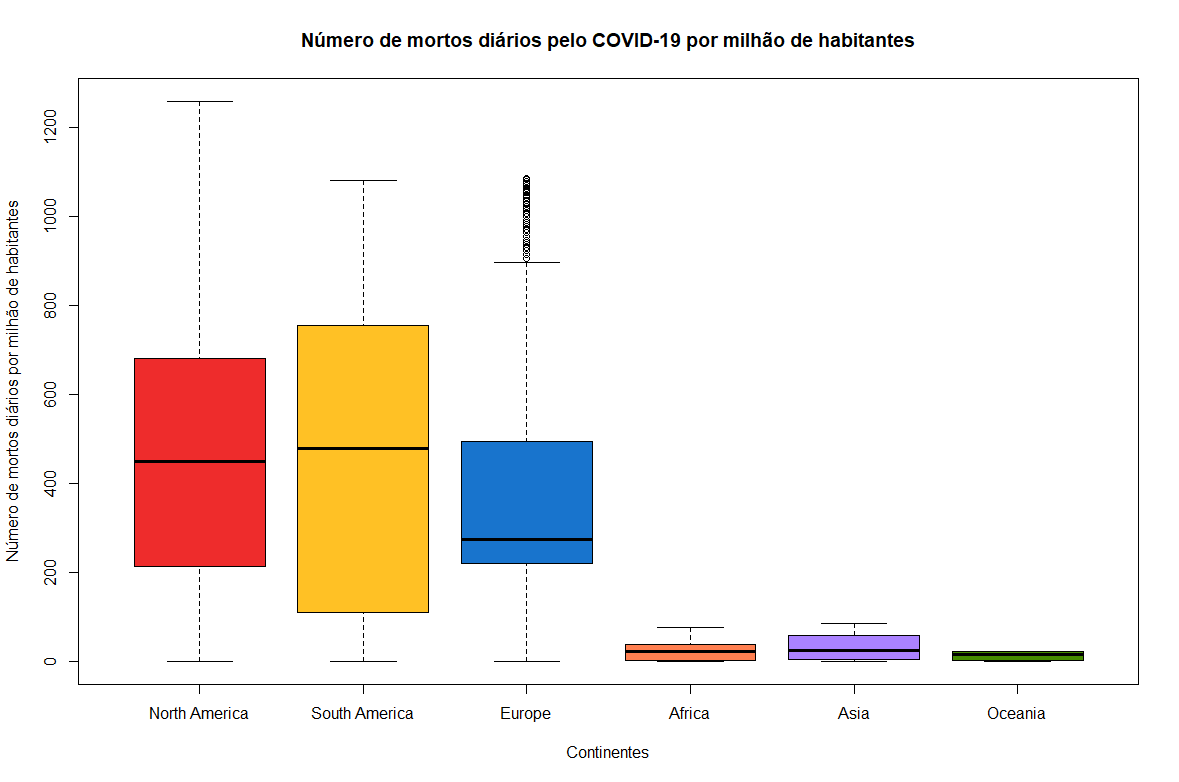
\includegraphics[width=0.95\columnwidth]{images/01.g.png}}
\caption{Diagrama de Caixa representativo do número de mortos diários pelo COVID-19 por milhão de habitantes, por continente}
\label{1g}
\end{figure}

O diagrama de caixa representado na Fig.\ref{1g} permite-nos afirmar que a América do Norte é o continente com maior número de mortos diários por milhão de habitantes.

A América do Sul é o continente mais disperso, visto que o tamanho da caixa (amplitude interquartil) é maior, comparativamente às restantes caixas, havendo, consequentemente, uma maior variação dos dados neste continente.

Analisando o fator de simetria, os dados da América do Norte e África são os que aparentam ter uma distribuição mais simétrica, dado que a linha da mediana se encontra posicionada no centro da caixa. Já a Europa e a Ásia denotam uma grande assimetria, sendo os seus dados assimetricamente negativos, uma vez que a linha da mediana se aproxima do primeiro quartil. A América do Sul e Oceânia também denotam uma assimetria, mas positiva, visto que a linha da mediana está mais próxima do terceiro quartil, contudo, a assimetria presente na América do Sul não é tão elevada.

\begin{equation}
x\in [Q1-1.5\times IQR, Q3+1.5\times IQR]\label{outlierCriteria}
\end{equation}

Por último, a Europa, mesmo depois de serem removidos alguns \textit{outliers} pelo critério x é \textit{outliers} se e só se satisfizer o critério indicado na equação \eqref{outlierCriteria}, é o continente que ainda apresenta bastantes valores discrepantes, estando estes acima do limite máximo.


\section{Análise Inferencial} % ------------------------------------------------------
A análise inferencial incidiu na geração de amostras pseudoaleatórias, com diferentes \textit{seeds} indicadas em cada alínea, para análise e verificação de diferenças significativas da taxa de transmissibilidade em Portugal e no Reino Unido, no número de mortes diárias em quatro países europeus e no número médio diário de mortes por continente. Estes dados são referentes ao período de 01 de abril de 2020 a 27 de fevereiro de 2021.

\subsection{Verificação se a média da taxa transmissibilidade no Reino Unido é superior à média da taxa de transmissibilidade em Portugal, relativamente aos dados de 30 dias}

\begin{figure}[htbp]
\centerline{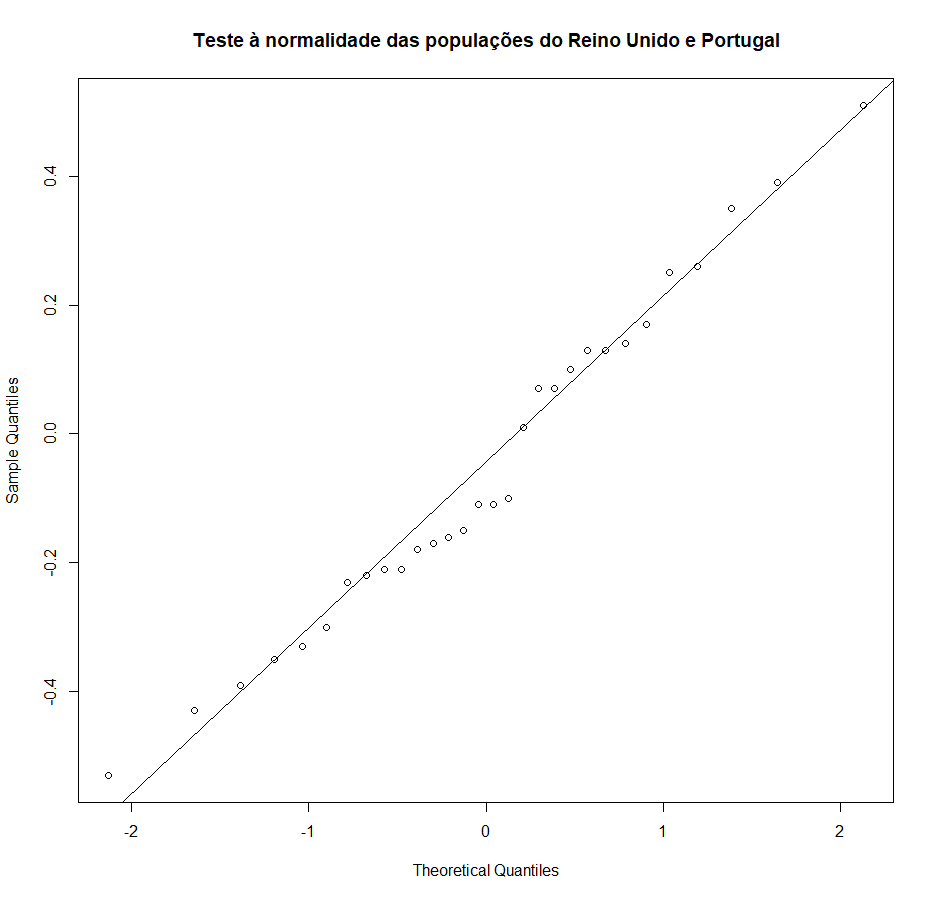
\includegraphics[width=0.95\columnwidth]{images/02.a.png}}
\caption{Diagrama de Dispersão representativo do teste à normalidade das populações do Reino Unido e Portugal}
\label{2a}
\end{figure}

\begin{equation}
  \begin{array}{l}
    H_{0}:\mu _{uk}\leq \mu _{pt} \\
   	H_{1}:\mu _{uk}> \mu _{pt}
  \end{array}\label{hipothesis2a}
\end{equation}

O teste de hipóteses segue a definição em \eqref{hipothesis2a}. Como os dados são relativos a 30 dias, e utilizada uma \textit{seed} de 118, pode-se concluir que as amostra de ambos os países seguem uma distribuição aproximadamente normal, através do Teorema do Limite Central, sendo que esta conclusão foi verificada com os testes de Shapiro-Wilk (p-value = 0.686), Lillierfors (p-value = 0. 1533) e, também, pelo método gráfico (representado na Fig.\ref{2a}), que demonstra que as variáveis têm uma relação linear. 

Ao saber que as distribuições são normais e são emparelhadas, uma vez que partilham a variável dos dias, realizou-se um t-Test que obteve um p-value igual a 0.8652, que permite concluir que não se deve rejeitar a hipótese nula, ou seja, que as médias das taxas de transmissibilidade dos dois países são idênticas, a um nível de significância superior a 8.5\%. Logo, a média da taxa de transmissibilidade do Reino Unido é semelhante à média registada em Portugal.


\subsection{Verificação da existência de diferenças significativas no número de mortes diárias, por milhão de habitantes, em Espanha, França, Portugal e Itália}
\begin{equation}
  \begin{array}{l}
    H_{0}:No.Deaths_{Spain}=No.Deaths_{France}= \\
    =No.Deaths_{Portugal}=No.Deaths_{Italy} \\
    H_{1}:No.Deaths_{Spain}\neq No.Deaths_{France}\neq \\
    \neq No.Deaths_{Portugal}\neq No.Deaths_{Italy}
  \end{array}\label{hipothesis2b}
\end{equation}

O teste de hipóteses segue a definição em \eqref{hipothesis2b}. Nesta análise foram utilizados 15 dias aleatórios e uma \textit{seed} de 115. Procedeu-se à realização de um teste de Friedman, uma vez que dispomos de n x k observações (sendo n os dias e k os países), com o objetivo de perceber se as amostras apresentam diferenças significativas. A escolha deste teste deve-se a possuírmos quatro amostras emparelhadas, uma vez que os dados dos diversos países têm os dias em comum.

O p-value obtido foi de 0.06018, que, por ser superior a 0.05, permite-nos aceitar a hipótese nula e concluir que não há diferenças significativas no número de mortes diárias por milhão de habitantes nestes quatro países.


\subsection{Verificação da existência de diferenças significativas nos números médios diários de mortes, por milhão de habitantes, entre os continentes}

\begin{equation}
  \begin{array}{l}
    H_{0}:\mu _{Asia}=\mu _{Africa}=\mu _{Europe}=\mu _{North America}= \\
    = \mu _{South America} \\ 
    H_{1}:\mu _{i}\neq \mu _{j}, i,j\in [Asia, Africa, Europe, \\
    North America, South America]
  \end{array}\label{hipothesis2c}
\end{equation}

\begin{equation}
	\begin{array}{l}
	Asia_{p-value}=0.07204, \\
	Africa_{p-value}=0.001552, \\
	Europe_{p-value}=0.001734, \\
	North America_{p-value}=0.08603, \\
	South America_{p-value}=2.932\times 10^{-8}
	\end{array}\label{pvalues2c1}
\end{equation}

O teste de hipóteses segue a definição em \eqref{hipothesis2c}. Nesta análise foram utilizadas \textit{seeds} de 100 a 104 referentes aos quatro continentes. Realizaram-se testes de Shapiro-Wilk para verificar a normalidade dos dados referentes a cada continente sendo que os resultados obtidos nos valores dos p-values \eqref{pvalues2c1} demonstram que Ásia, Europa e América do Sul não seguem distribuições normais uma vez que os seus p-values são inferiores a 0.05, rejeitando, assim, a hipótese nula.

\begin{equation}
p-value = 1.437\times 10^{-11}\label{pvalue2c2}
\end{equation}

Após estas confirmações realizou-se um teste Levene para verificar a homogeneidade dos dados, sendo que o valor obtido do p-value \eqref{pvalue2c2} permite concluir que as variâncias dos dados são significativamente diferentes.

\begin{equation}
p-value < 2\times 10^{-16}\label{pvalue2c3}
\end{equation}

Com os resultados destes testes, realizou-se um teste ANOVA, ainda que o teste de Levene tenha indicado que as variâncias sejam diferentes, sendo que se obteve um p-value \eqref{pvalue2c3} reduzido e inferior a 0.05.

Isto permite concluir que se deve rejeitar a hipótese nula, ou seja, que não existe igualdade entre os números médios de mortos diários, por milhão de habitantes, entre os continentes.

\begin{figure}[htbp]
\centerline{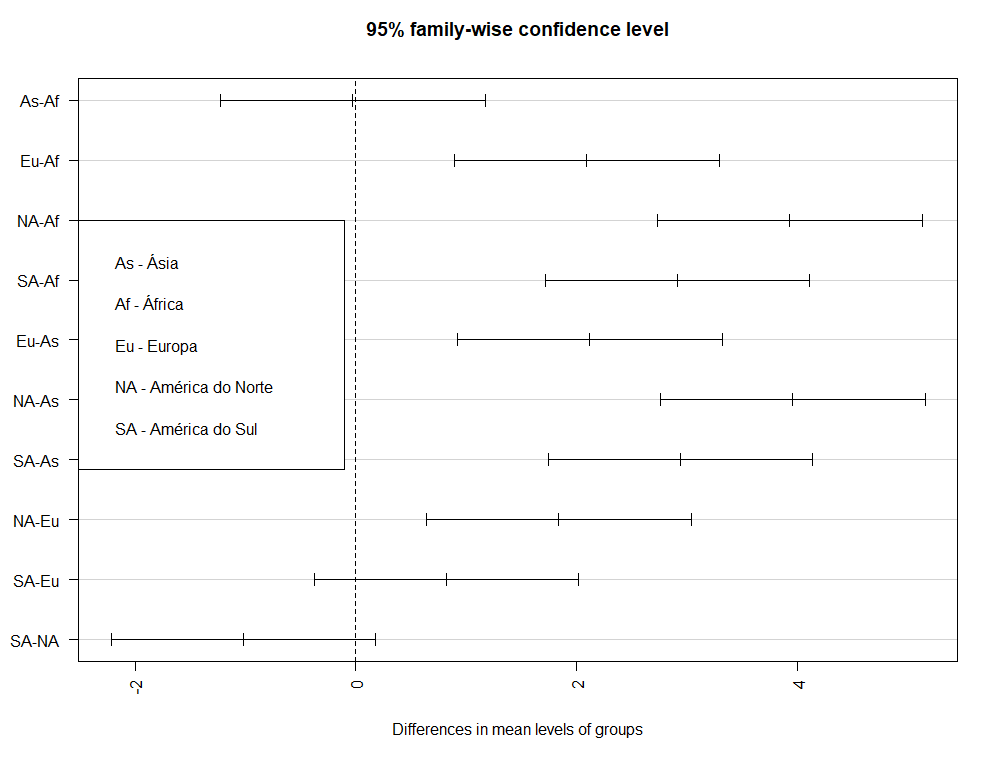
\includegraphics[width=0.95\columnwidth]{images/02.c.png}}
\caption{Gráfico representativo dos Intervalos de Confiança para a diferença das médias dos dados, entre os continentes}
\label{2c}
\end{figure}

Após a realização e conclusões retiradas com o teste ANOVA, realizou-se um teste post-hoc \cite{posthoc} com o objetivo de perceber mais sobre as diferenças das médias dos dados entre os continentes. Assim sendo, realizou-se um teste Tukey’s Honest Significant Difference \cite{tukey}, com o qual se obteve os dados apresentados na Fig.\ref{2c}.

Através do gráfico, é possível verificar que as médias da Ásia-África são estatisticamente semelhantes, uma vez que o intervalo de confiança contém o valor nulo. O mesmo acontece com as médias da América do Sul-Europa e América do Norte-América do Sul, no entanto carecem da mesma expressividade de igualdade relativamente à relação dos outros dois continentes, uma vez que, apesar do 0 se encontrar dentro dos intervalos, descai para os seus extremos.

Em relação às outras relações existentes, conclui-se que estas apresentam diferenças significativas nas médias, onde os continentes da Europa, América do Norte e América do Sul apresentam média superiores às de África e Ásia.


\section{Análise de Correlação} % ------------------------------------------------------
Nesta análise pretende-se averiguar, em 2021, a existência de correlação entre dados referentes a países europeus com mais de 10 milhões de habitantes, nomeadamente o valor máximo da taxa de transmissibilidade, a densidade populacional, o total de mortos e a percentagem da população com 65 ou mais anos.

\subsection{Correlação, em 2021, entre o valor máximo da taxa diária de transmissibilidade e a densidade populacional de todos os países da Europa com mais de 10 milhões de habitantes}

Sendo X1 a variável representativa do valor máximo da taxa diária de transmissibilidade de todos os países europeus com mais de 10 milhões de habitantes e Y1 da densidade populacional dos mesmos, foram verificados, em primeiro lugar, os seguintes pressupostos:

\subsubsection{As variáveis devem ser contínuas e não devem existir outliers significativos}

\begin{figure}[htbp]
\centerline{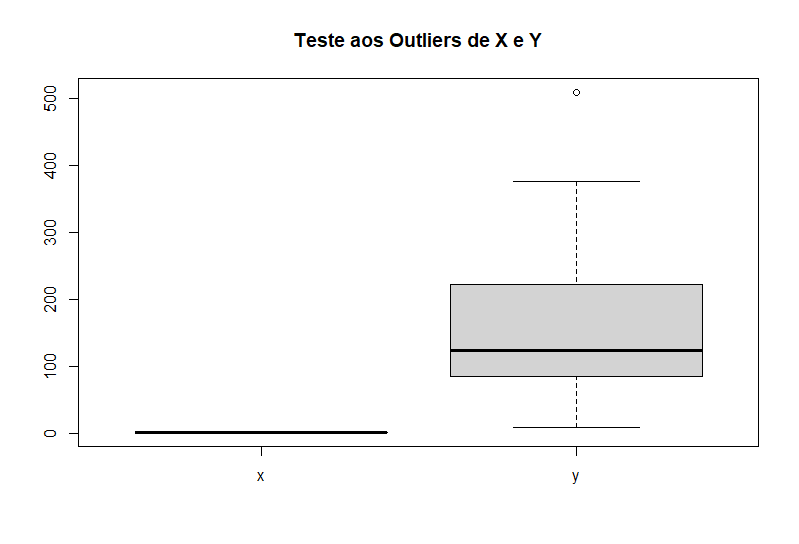
\includegraphics[width=0.95\columnwidth]{images/03.a.1.png}}
\caption{Diagrama de Caixa representativo das variáveis X1 e Y1}
\label{3a1}
\end{figure}

Sendo as variáveis contínuas, pretendeu-se verificar, através de um diagrama de caixa, se os outliers seriam significativos, o que se conclui pelo gráfico da Fig.\ref{3a1} que não o são.

\subsubsection{Deve existir uma relação linear entre as duas variáveis}

\begin{figure}[htbp]
\centerline{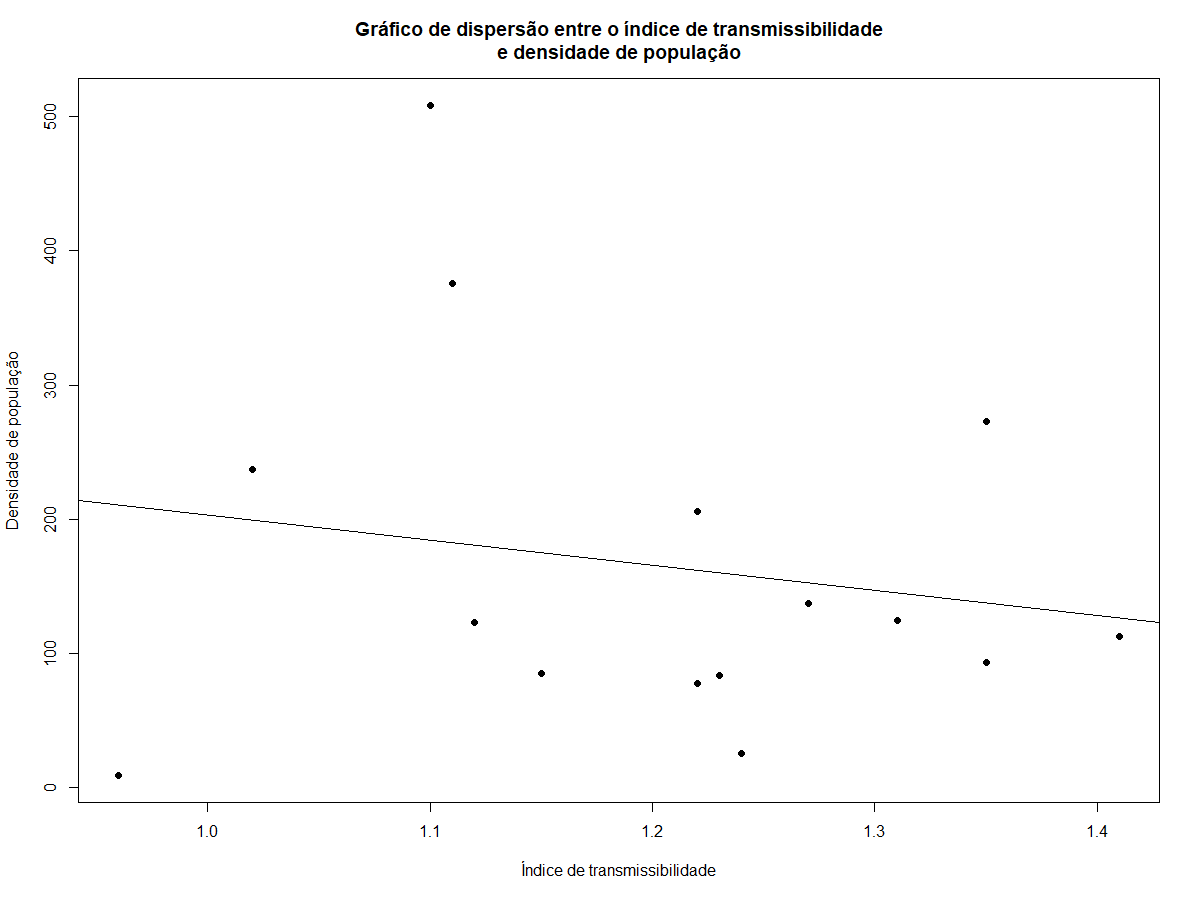
\includegraphics[width=0.95\columnwidth]{images/03.a.2.png}}
\caption{Diagrama de Dispersão representativo das variáveis X1 e Y1}
\label{3a2}
\end{figure}

Para a confirmação desta condição realizou-se um diagrama de dispersão (Fig.\ref{3a2}) onde se comprova que não existe uma relação linear entre as duas variáveis, estando os pontos demasiado dispersos em relação à linha traçada. Este pressuposto não é, então, verificado.

\subsubsection{As variáveis devem ter, aproximadamente, uma distribuição normal}

\begin{figure}[htbp]
\centerline{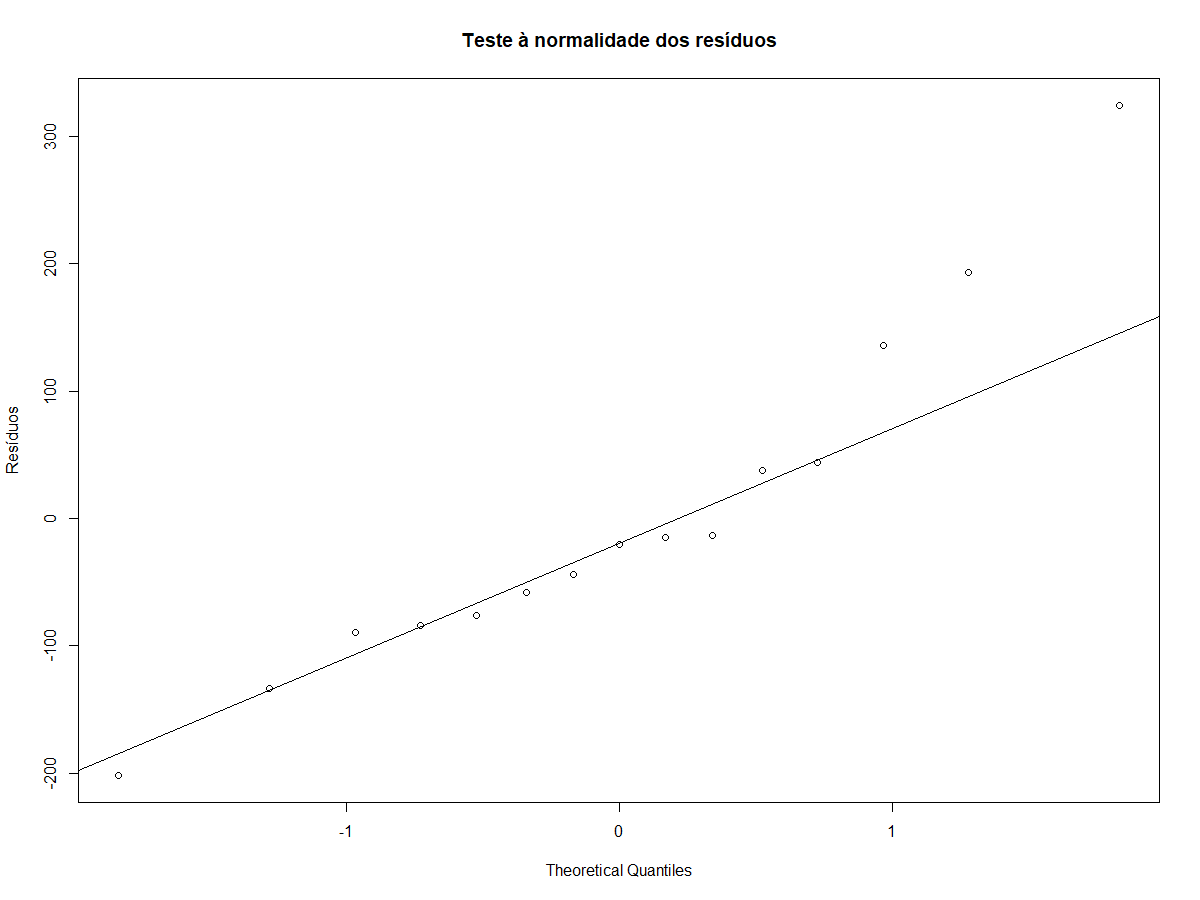
\includegraphics[width=0.95\columnwidth]{images/03.a.3.png}}
\caption{Gráfico de Dispersão Normal Q-Q representativo das variáveis X1 e Y1}
\label{3a3}
\end{figure}

Ao realizar um gráfico de dispersão Normal Q-Q (Fig.\ref{3a3}), verificam-se que os pontos estão razoavelmente ajustados à linha reta, o que nos permite a suspeita dos resíduos serem normais. Pelo teste de normalidade Shapiro-Wilk, obteve-se um p-value de 0,2014, pelo que se confirma a condição de normalidade, já que este é superior a 0,05.

\subsubsection{As variâncias devem ser iguais (Homocedasticidade)}

\begin{figure}[htbp]
\centerline{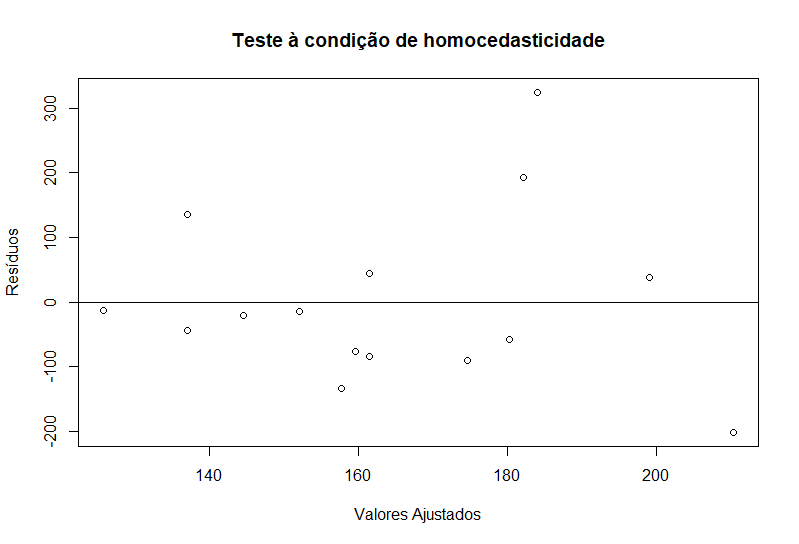
\includegraphics[width=0.95\columnwidth]{images/03.a.4.png}}
\caption{Diagrama de Dispersão ajustado representativo das variáveis X1 e Y1}
\label{3a4}
\end{figure}

Por fim, no gráfico de dispersão da Fig.\ref{3a4} não se denota qualquer tendência no mesmo, estando os pontos aleatoriamente distribuídos em torno do valor 0, onde se traçou uma linha. Assim, temos indícios de que a variância dos resíduos é homocedástica, contudo, sendo a amostra pequena (x e y = 15 < 30), testou-se também a variância. No teste à variância o p-value obtido é ligeiramente acima de 0,05 (0,05919), o que nos permite aceitar a análise anterior e concluir que as variâncias são iguais.

Verificados três dos pressupostos anteriores, procedeu-se à realização de um Teste de Correlação Linear de Pearson, onde se concluiu que, de facto, as variáveis estão fracamente correlacionadas, uma vez que o valor de r obtido é próximo de 0 (-0,175886) e o valor de p-value não é significativo, estando bastante acima de 0,05 (0,5306).

\subsection{Correlação, em 2021, entre o total de mortos por milhão de habitantes e a percentagem da população com 65 anos ou mais em todos os países da Europa com mais de 10 milhões de habitantes}

Primeiramente foram verificados os seguintes pressupostos:

\subsubsection{As variáveis devem ser contínuas e não devem existir outliers significativos}

\begin{figure}[htbp]
\centerline{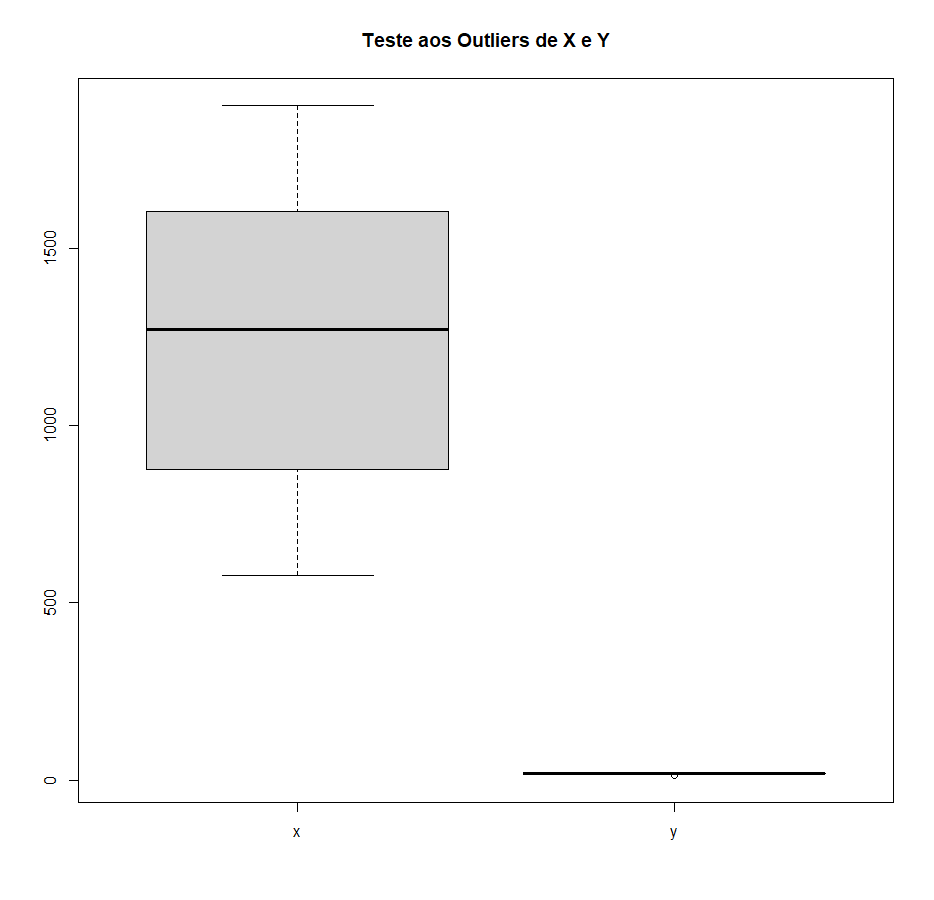
\includegraphics[width=0.95\columnwidth]{images/03.b.1.png}}
\caption{Diagrama de Caixa representativo das variáveis X2 e Y2}
\label{3b1}
\end{figure}

Como as variáveis são contínuas, verificou-se, através de um diagrama de caixa, se os outliers seriam significativos, o que se conclui pelo gráfico da Fig.\ref{3b1} que não o são.

\subsubsection{Deve existir uma relação linear entre as duas variáveis}

\begin{figure}[htbp]
\centerline{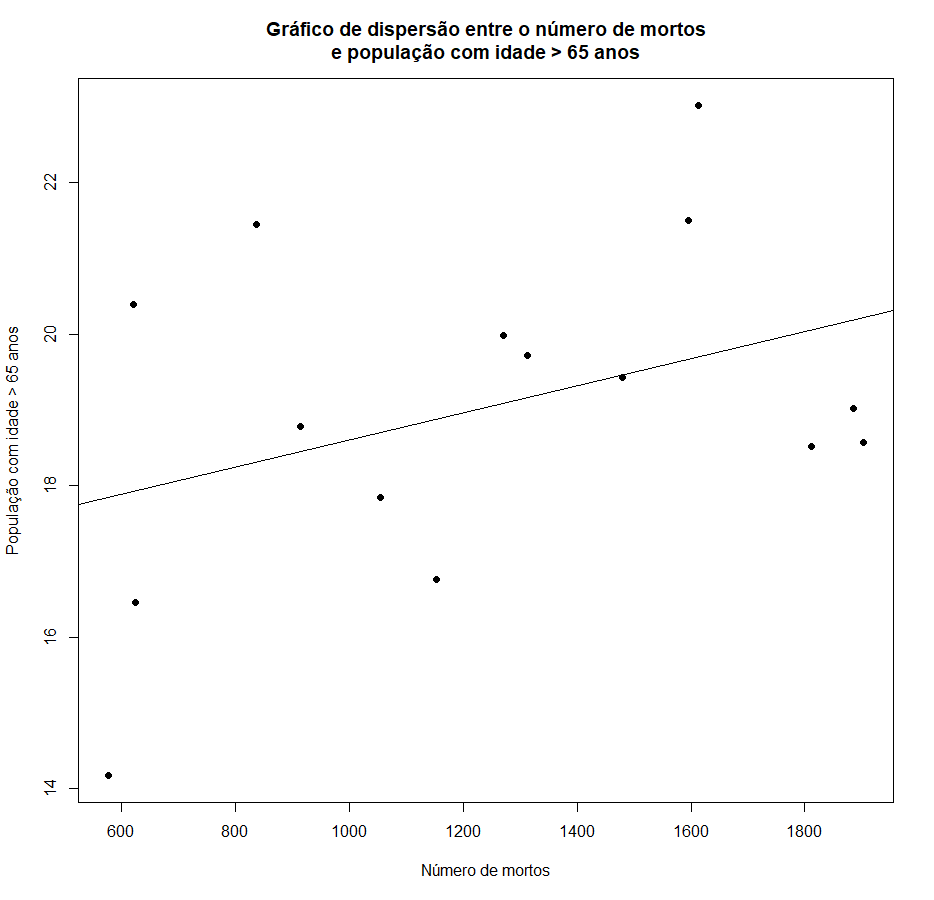
\includegraphics[width=0.95\columnwidth]{images/03.b.2.png}}
\caption{Diagrama de Dispersão representativo das variáveis X2 e Y2}
\label{3b2}
\end{figure}

Através do diagrama de dispersão (Fig.\ref{3b2}) comprova-se que não existe uma relação linear entre as duas variáveis, uma vez que os pontos se encontram distantes da linha de regressão traçada.

\begin{figure}[htbp]
\centerline{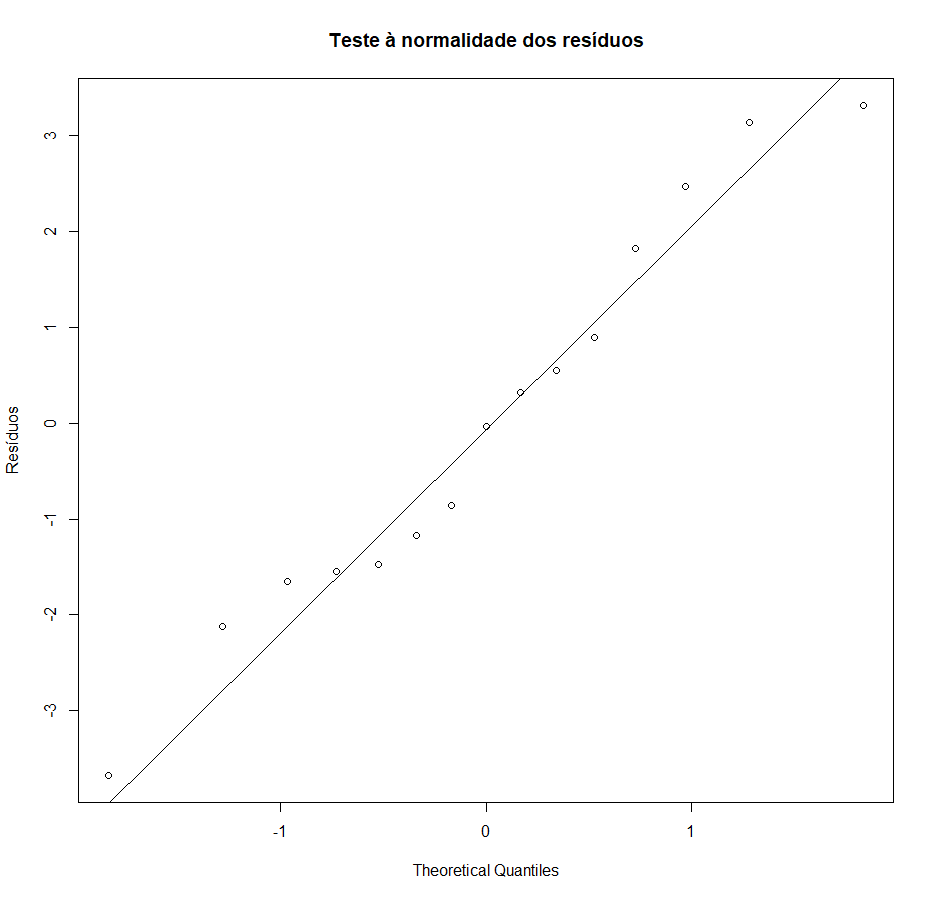
\includegraphics[width=0.95\columnwidth]{images/03.b.3.png}}
\caption{Gráfico de Dispersão Normal-QQ representativo das variáveis X2 e Y2}
\label{3b3}
\end{figure}

Ao realizar um gráfico de dispersão Normal Q-Q (Fig.\ref{3b3}), verificam-se que os pontos estão ajustados à linha reta, ou seja, permite concluir que os resíduos seguem uma distribuição normal.

\subsubsection{As variáveis devem ter, aproximadamente, uma distribuição normal}

Pelo teste de Shapiro-Wilk, obteve-se um p-value de 0,7183, que confirma a condição de normalidade, obtendo a mesma conclusão do método gráfico.

\subsubsection{As variâncias devem ser iguais (Homocedasticidade)}

\begin{figure}[htbp]
\centerline{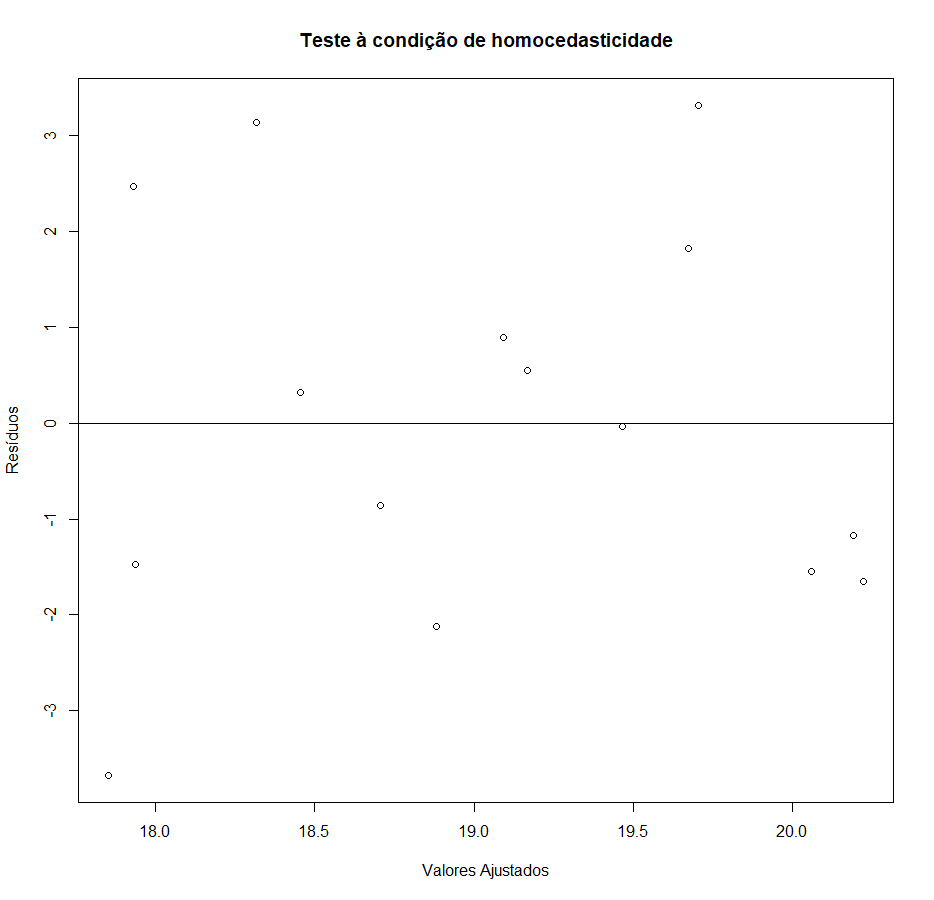
\includegraphics[width=0.95\columnwidth]{images/03.b.4.png}}
\caption{Diagrama de Dispersão ajustado representativo das variáveis X2 e Y2}
\label{3b4}
\end{figure}

Por fim, no gráfico da Fig.\ref{3b4} não se denota qualquer tendência no gráfico, estando os pontos aleatoriamente distribuídos em torno do valor 0, onde se traçou uma linha. Assim, temos indícios de que a variância dos resíduos é homocedástica, contudo, sendo a amostra pequena (x = y = 15 < 30), testou-se também a variância.

No teste à variância o p-value obtido é ligeiramente acima de 0,05 (0,05919), o que nos permite aceitar a análise anterior e concluir que as variâncias são iguais.


Verificados três dos pressupostos anteriores, procedeu-se à realização de um Teste de Correlação Linear de Pearson.

De facto, as variáveis estão fracamente correlacionadas, uma vez que o valor de r obtido é próximo de 0 (-0,175886) e o valor de p-value não é significativo, estando bastante acima de 0,05 (0,5306).


\section{Análise de Regressão} % ------------------------------------------------------
Na análise de regressão considerou-se o "Índice de rigor" médio mensal (Ir) em Portugal, a variável dependente e as variáveis independentes: média de mortes diárias por milhão de habitantes (Dm), média de casos diários por milhão de habitantes (Cm) e a média mensal da taxa de transmissibilidade (Rm). Os dados foram considerados no período entre 01 de abril de 2020 e 27 de fevereiro de 2021.

\subsection{Construção do modelo de regressão linear múltipla}

\begin{equation}
\begin{array}{l}
	Y=\beta _{0}+\beta _{1}X_{1}+\beta _{1}X_{3}+\beta _{3}X_{3} \\
	\beta _{0}=81.827720 \qquad \beta _{0 p-value}=2\times 10^{-16} \\
	\beta _{1}=0.139378 \qquad \beta _{1 p-value}=0.141 \\
	\beta _{2}=0.002183 \qquad \beta _{2 p-value}=0.259 \\
	\beta _{3}=-9.096406 \qquad \beta _{3 p-value}=8.55\times 10^{-16}
\end{array}\label{lrm}
\end{equation}

O modelo de regressão linear obtido através das variáveis independentes: mortes diárias, casos diários e taxa de transmissibilidade; para a variável dependente índice de rigor resulta na equação em \eqref{lrm} com os valores dos coeficientes obtidos.

Relativamente à significância dos coeficientes obtidos, a interseção e a taxa de transmissibilidade são aqueles que apresentam p-values extremamente  baixos, sendo estatisticamente significantes, enquanto os coeficientes das mortes diárias e casos diários apresentam um p-value alto, de 0.141 e 0.259, respetivamente, ou seja, são valores com baixo nível de significância estatisticamente.

\begin{equation}
	R^{2}_{ajustado}=0.2275 \label{r2}
\end{equation}
\begin{equation}
	Estatistica _{p-value}=2.2\times 10^{-16} \label{pvalue4a}
\end{equation}

O valor do R-quadrado ajustado \eqref{r2} indica que apenas 22.75\% dos valores do Índice de Rigor são explicados pelos outros parâmetros. Como o valor do p-value da estatística de teste \eqref{pvalue4a} é bastante reduzido, o valor do R-quadrado ajustado é estatisticamente significativo.

\subsection{Verificação da satisfação das condições de Homocedasticidade, Autocorrelação nula e de Multicolinearidade}

\subsubsection{Homocedasticidade} 

\begin{equation}
p-value = 6.232\times 10^{-13}\label{pvalue4b1}
\end{equation}

Ao realizar um gráfico Normal Q-Q denota-se uma certa tendência linear nos pontos, levantando a suspeita de que a distribuição dos resíduos não é normal, o que se confirma pelo teste de Shapiro que adquire um p-value inferior a 0,05 \eqref{pvalue4b1}.

\begin{equation}
p-value = 2.2\times 10^{-16}\label{pvalue4b2}
\end{equation}

Para além de não se confirmar a normalidade dos resíduos, confirmou-se ainda através de um t.test que a média dos erros não é zero e, através de um teste à variância, que comprovou também que as variâncias não são constantes, já que o p-value é inferior a 0,05 \eqref{pvalue4b2}.

\subsubsection{Autocorrelação Nula} 
Para verificar esta condição recorreu-se a um teste de Durbin Watson, sendo as hipóteses testadas as seguintes:

H0: Os resíduos são independentes.

H1: Os resíduos não são independentes.

Obtendo um p-value de 0, sendo este inferior a 0.05, rejeita-se a hipótese nula, o que nos permite afirmar que a condição de independência não se verifica.

\subsubsection{Multicolinearidade} 

\begin{equation}
\begin{array}{l}
	D_{m}=5.744092 \\
	C_{m}=5.665572 \\
	R_{m}=1.715799
\end{array} \label{DmCmRm}
\end{equation}

Por último, foi testada a multicolinearidade dos resíduos pelo Fator de Inflação de Variância (VIF), sendo que se considera a ausência de multicolinearidade quando o VIF é inferior a 3. Através deste teste, cujos valores obtidos estão apresentados em \eqref{DmCmRm}, verificou-se que Dm e Cm são multicolineares, contrariamente a Rm.


\subsection{Estimação do Ir para os valores Dm = 10, Cm = 460, Rm = 1.1}
A estimação do valor do Índice de Rigor médio mensal para os valores de Dm = 10, Cm = 460, Rm = 1.1 resulta num índice de 74.21956, com um nível de confiança de 95\%, pertencente ao intervalo de confiança [73.52288, 74.91623].


\section{Conclusões} % ------------------------------------------------------
Através da análise exploratória constata-se que a América do Norte e a Europa são os continentes que mais se evidenciam, quer no número de infetados, quer no número de mortes, registando os valores mais elevados. Em contrapartida, a Oceânia demonstra ser o continente menos afetado pelo COVID-19, assinalando os menores valores.

Da inferência estatística conclui-se que a média da taxa de transmissibilidade do Reino Unido é semelhante à média registada em Portugal. De igual modo, também se verificou não existirem diferenças significativas no número de mortes diárias, por milhão de habitantes, em Espanha, França, Portugal e Itália. Por fim, constatou-se a existência de diferenças significativas no número médio de mortos diários, por milhão de habitantes, entre os vários continentes, sendo a Ásia e África aqueles com menores médias, excluindo a Oceânia, uma vez que registou os números mais baixos comparativamente ao resto do mundo.

Relativamente à análise de correlação, observou-se que ambas as análises estão fracamente correlacionadas, obtendo valores de relação próximos do 0 e de p-value não significativos. Denotou-se também que ambas falharam no mesmo pressuposto, sendo este o critério da existência de uma relação linear entre as duas variáveis, o que previu a falta de correlação entre os dados de cada análise.

Finalmente, na análise de regressão demonstrou-se que a relação linear múltipla não é muito forte, sendo que apenas a variável independente Rm possui uma relação linear com a variável dependente (Ir), contrariamente às restantes. Este fator foi comprovado quer na construção do modelo de regressão linear múltipla, quer na verificação da condição de multicolinearidade. Consequentemente, existe uma falta de precisão das previsões de valores do Ir através dos valores das variáveis independentes.

\begin{thebibliography}{00}

\bibitem{database} Ritchie, H. (2021, 3 de abril). \textit{Coronavirus Source Data}. Our World in Data. \url{https://ourworldindata.org/coronavirus-source-data}

\bibitem{dataFile} Our World in Data (2021, 3 de abril). [Ficheiro Csv]

\bibitem{nortest} Gross, J. \& Ligges, U. (2015, 30 de julho). \textit{nortest: Tests for Normality}. R Project. \url{https://cran.r-project.org/web/packages/nortest/index.html}

\bibitem{car} Fox, J. \& Outros (2020, 29 de setembro). \textit{car: Companion to Applied Regression}. R Project. \url{https://cran.r-project.org/web/packages/car/index.html}

\bibitem{colors} Department of Statistics (2021, 3 de abril). \textit{Colors in R}. Columbia University. \url{http://www.stat.columbia.edu/~tzheng/files/Rcolor.pdf?utm_source=twitterfeed&utm_medium=twitter}

\bibitem{posthoc} Autor desconhecido (2020, 17 de agosto). \textit{Post Hoc Tests}. LibreTexts Statistics. \url{https://stats.libretexts.org/Bookshelves/Applied_Statistics/Book\%3A_An_Introduction_to_Psychological_Statistics_(Foster_et_al.)/11\%3A_Analysis_of_Variance/11.08\%3A_Post_Hoc_Tests}

\bibitem{tukey} Frost, J. (2021, 22 de abril). \textit{Using Post Hoc Tests with ANOVA}. Statistics By Jim. \url{https://statisticsbyjim.com/anova/post-hoc-tests-anova/}

\end{thebibliography}

\end{document}
